% Chapter 3

\chapter{Assembling the battery} % Main chapter title

\label{chap3} % For referencing the chapter elsewhere, use \ref{Chapter1} 

%----------------------------------------------------------------------------------------

% Define some commands to keep the formatting separated from the content 
%----------------------------------------------------------------------------------------

\section{Formation of slurry}
To make a slurry, we mixed together the active material, conductive carbon and a binder, PVDF, all together in a glass vial. It is important for the slurry to be homogeneous. This helps in the coating process at  later stages. A binder (an inert material) is used to help hold together the active material on a current collector. It has been seen adding a binder reduces the conductivity of the active material. To compensate for this loss, a super-conductive carbon (Super-P) is added to the slurry. Polyvinylidene fluoride (PVDF) is mixed separately in an organic solvent, N-methyl pyrrolidinone (NMP). This viscous solution is added to the mixture of active material and Super-P. NMP can be added at later stages to adjust the consistency of the slurry. It is then mixed on a magnetic stirrer for 8-10 hours. Sometimes, an ultra-sonicator was used to prepare the slurries when the mixture did not form a well-dispersed solution. 

\section{Preparing a cathode}
Once the slurry is prepared, it is coated on a current collector. A current collector is a conductive solid part connected to the electrode with external loading. The main role of the current collector is to support the electrode and to collect the accumulated electrical energy from the electrode\cite{sun_effect_2017}. Initially, we used a  nickel foil as current collectors, but we found that Ni started oxidising itself at 1.0 V. This did not allow the cell to reach it's cut-off potential which was at 2.4 V. This not only hindered with the cell's redox processes, it also reduced the cell's capacity. After trial and error, we found that molybdenum foil had no effect whatsoever on the cell's behaviour (discussed in Appendix A). We established it as our current collector in all our battery systems discussed later. After coating the foils with the slurry, the electrodes were dried at 80$^{\circ}$C for two hours to improve the adhesion of the slurry. 
\begin{figure}[tbh!]
\centering
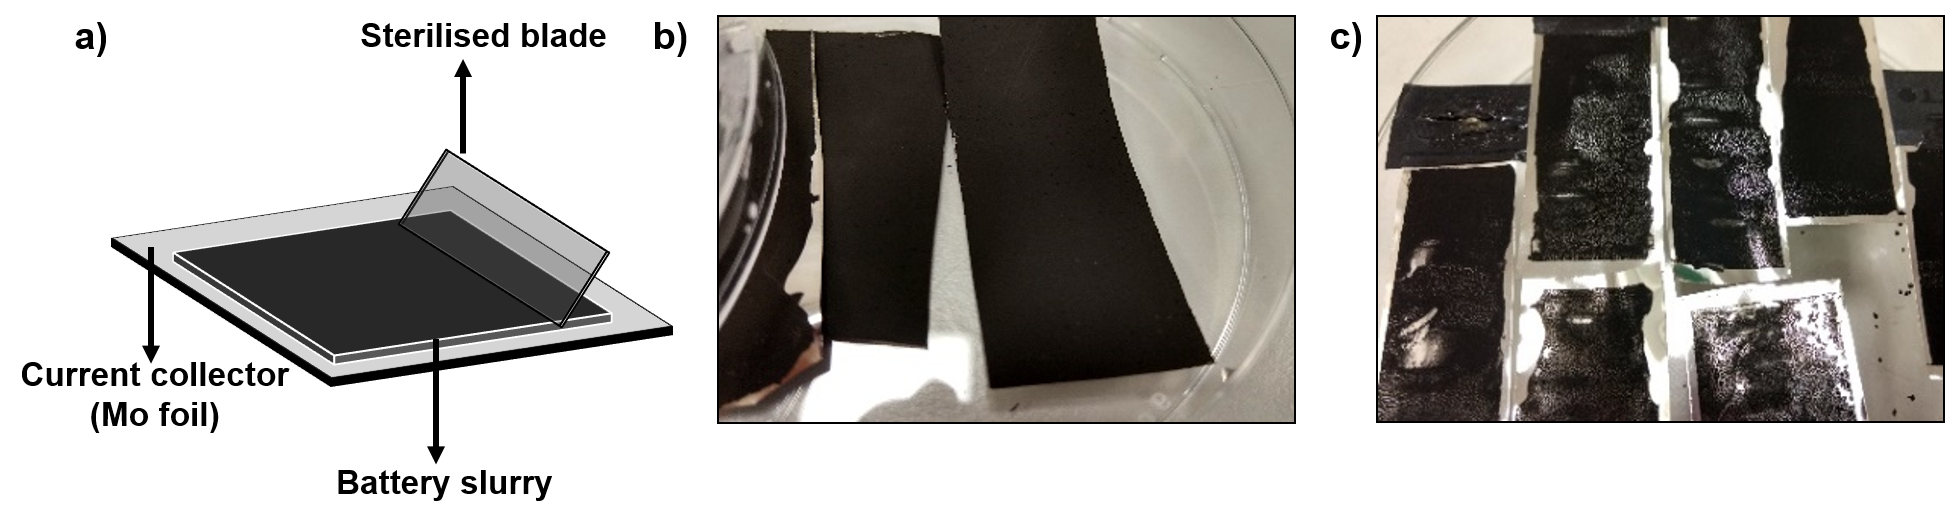
\includegraphics[width=\textwidth]{Figures/chap3fig/coating}
\caption{a) Slurry coating on a molybdenum foil using a steel blade, a process called doctor-blading. b) A uniformly coated cathode, and c) a non-uniform coated cathode}
\label{Figures/chap3fig:coating}
\end{figure}
\section{Vacuum drying}
Vacuum drying is a moisture-removal technique by means of creating a vacuum. Vacuum drying is used for the drying things which are hygroscopic (water sensitive) and heat sensitive. It creates vacuum to decrease the chamber pressure below the vapor pressure of the the solvent (NMP), causing it to boil. This decreases the boiling point of the solvent inside our electrodes and increases the rate of evaporation. It increases the drying rate of the product. The pressure maintained in vacuum drying is generally 0.03–0.06 atm. Thus, it is a drying process performed at reduced pressures and lower relative humidity compared to ambient pressure, enabling faster drying. Once the electrodes have been vacuum dried, they are ready to be used as cathodes in aluminium-ion batteries. 
\section{Assembling the cell}
Battery researchers generally use pouch cells or coin cells to test a cell's performance. CR-2032\textregistered\ cells have been predominantly used. Unfortunately, the ionic liquid used as the electrolyte in our cells reacted with the steel present in the coin cell components. We switched to custom-made cells that used PEEK (polyether ether ketone) for the main body and steel rods as the current collectors. PEEK  is a colourless organic thermoplastic polymer, used primarily for engineering applications. It has a melting point of 343$^{\circ}$C,  with excellent mechanical and chemical resistance properties that are retained at high temperatures. At room temperature, it remains inert to strong Bronsted and Lewis acids. Initially steel rods were used as current collectors, but because of their reactivity with the electrolyte we switched to molybdenum rods. 
\begin{figure}[tbh!]
\centering
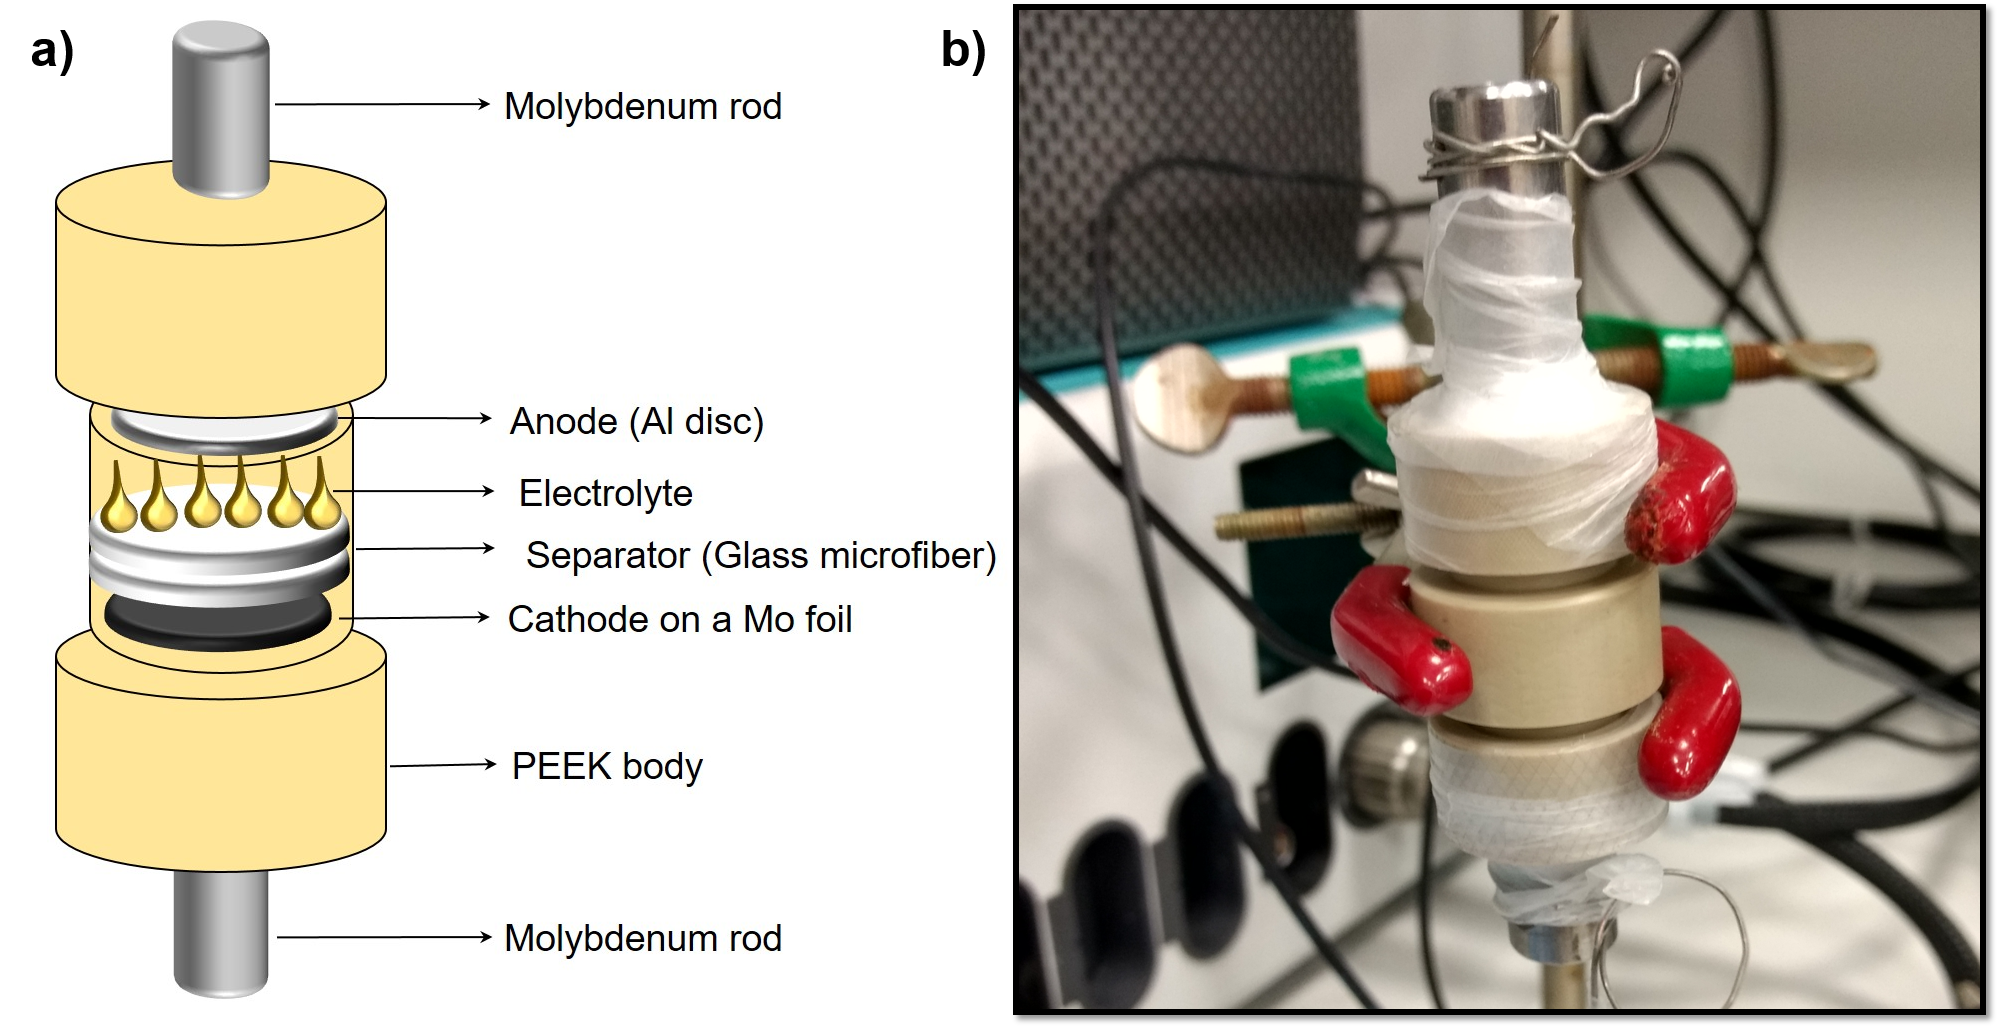
\includegraphics[width=\textwidth]{Figures/chap3fig/swagelok}
\caption{a) Assembly of a two-electrode PEEK cell using a cathode, separators wetted with electrolyte and an anode. Mo rods were used as plungers instead of steel and Mo foil was used as current collector instead of steel/Ni foil. b) A custom-made lab cell ready for preliminary electrochemical measurements.}
\label{Figures/chap3fig:swagelok}
\end{figure}
We first placed a cathode at the bottom of the cell, two separators made of glass microfibers were put above the cathode. The separators had been wetted in the electrolyte before being put in the cell. After that, a few drops of electrolyte (80 $\mu$l) were added into the cell. An anode made of pure aluminium was then placed on top and the cell was then sealed off. Since the electrolyte is highly hygroscopic, the entire cell was assembled inside a glove box with <0.1ppm \ce{O2},\ce{H2O}.
The cells were ready for electrochemical measurements as shown in Figure \ref{Figures/chap3fig:swagelok}. 





















